\subsubsection{Incremento 9}
\textit{\textbf{Periodo}: dal 2021-04-01 al 2021-04-13}

\myparagraph{Obiettivi}
Gli obiettivi definiti per questo incremento sono i seguenti:
\begin{itemize}
\item preparazione alla presentazione della Product baseline\ped{G};
\item incremento della documentazione.
\end{itemize}

\myparagraph{Attività}
Per raggiungere gli obiettivi, vengono svolte le seguenti attività:
\begin{itemize}
\item \textbf{presentazione Product baseline\ped{G}}: creazione e preparazione della presentazione con il \CR{} e con il proponente;
\item \textbf{ampliamento documentazione e verifiche}:
\begin{itemize}
\item incremento del \textit{\MU{}};
\item incremento del \textit{\MM{}};
\item completamento dell'\textit{Allegato tecnico}\ped{G} con i diagrammi mancanti;
\item incremento del \Glossariov{2.0.0};
\item rilevazione e registrazione di metriche, esiti di verifica e obiettivi di qualità;
\item aggiornamento dei rischi rilevati;
\item calcolo e registrazione del consuntivo di periodo.
\end{itemize}

\end{itemize}
\myparagraph{Diagramma di Gantt}
\begin{figure}[H]
\centering

\centerline{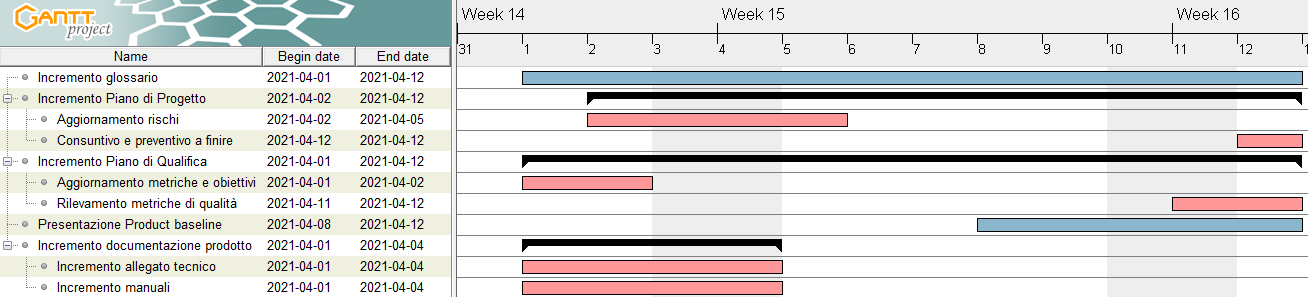
\includegraphics[scale=0.5]{res/Pianificazione/Fasi/CodificaIncrementi/ganttIncremento9}}
\caption{Diagramma di Gantt per l'incremento 9}
\end{figure}